
\section{Temporal Analysis}
\label{sec:temporal}

In this section, we study the temporal property of VirusTotal malwares. 

\begin{figure}[t!]
\begin{center}
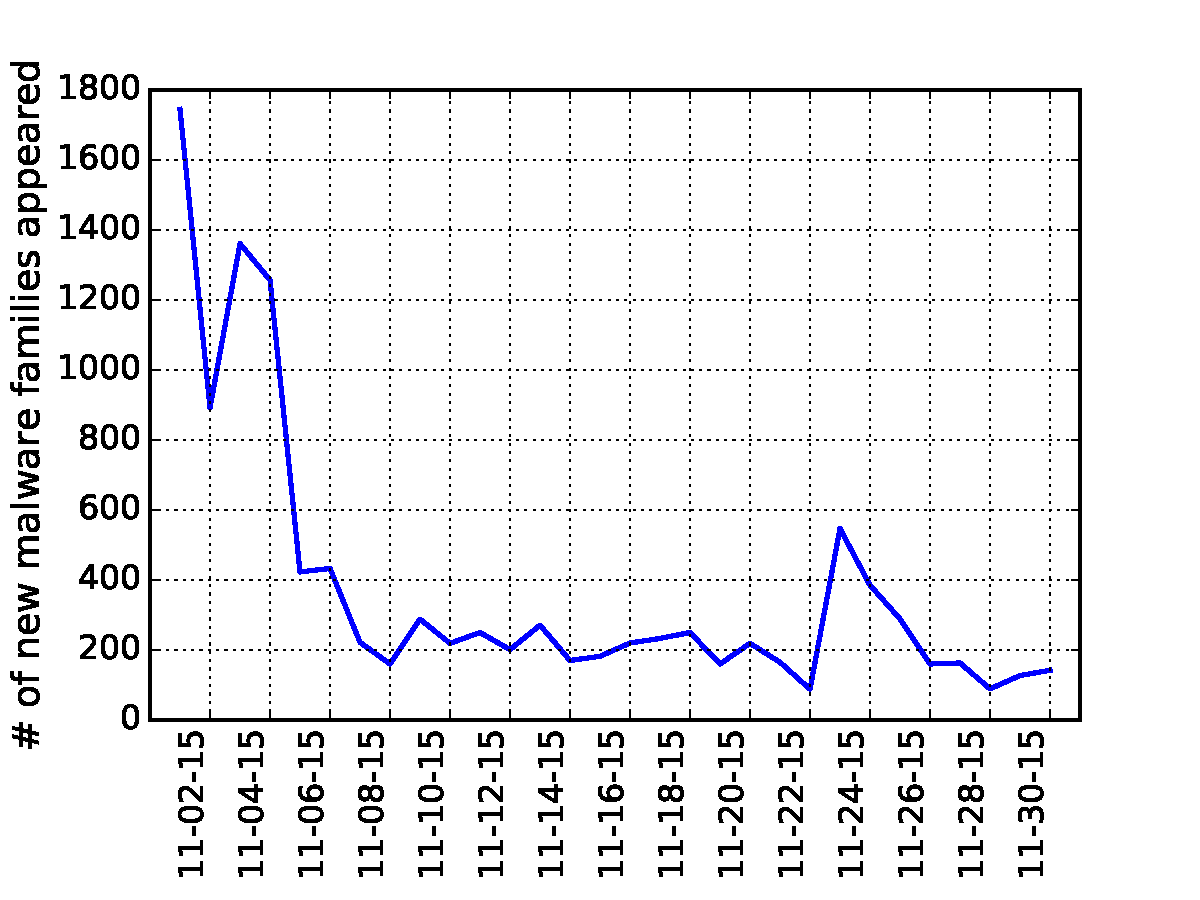
\includegraphics[width=2.5in]{figure/new_family}
\caption{The number of new malware families we observed each day in November 2015.}
\label{fig:new}
\end{center}
\end{figure}


We first study how many new malware families appear each day. 
Figure~\ref{fig:new} shows the number of new malware families appearing each day in November 2015. 
We do not have any data before November 1, 
so there are many more new malware families in the first few days.
After that, the number of new malware families becomes stable, falling into a range between 100 and 400. 
In total, there are 11311 malware families. 

{\bf Observation 1:} 
There are 100-400 new malware families appearing each day. 


\begin{figure}[t!]
\begin{center}
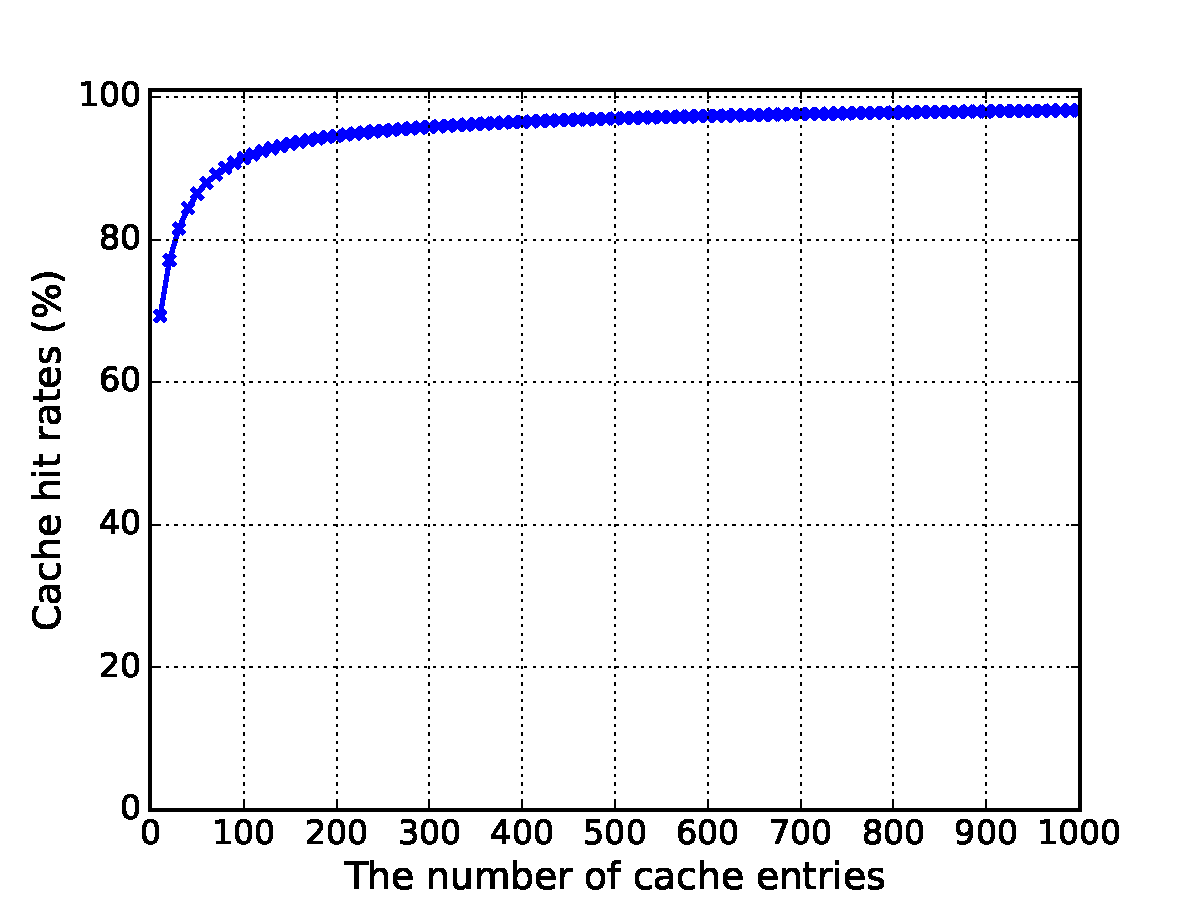
\includegraphics[width=2.5in]{figure/LRU}
\caption{Relation between cache hit rate and cache size.}
\label{fig:cache}
\end{center}
\end{figure}


\begin{figure}[t!]
\begin{center}
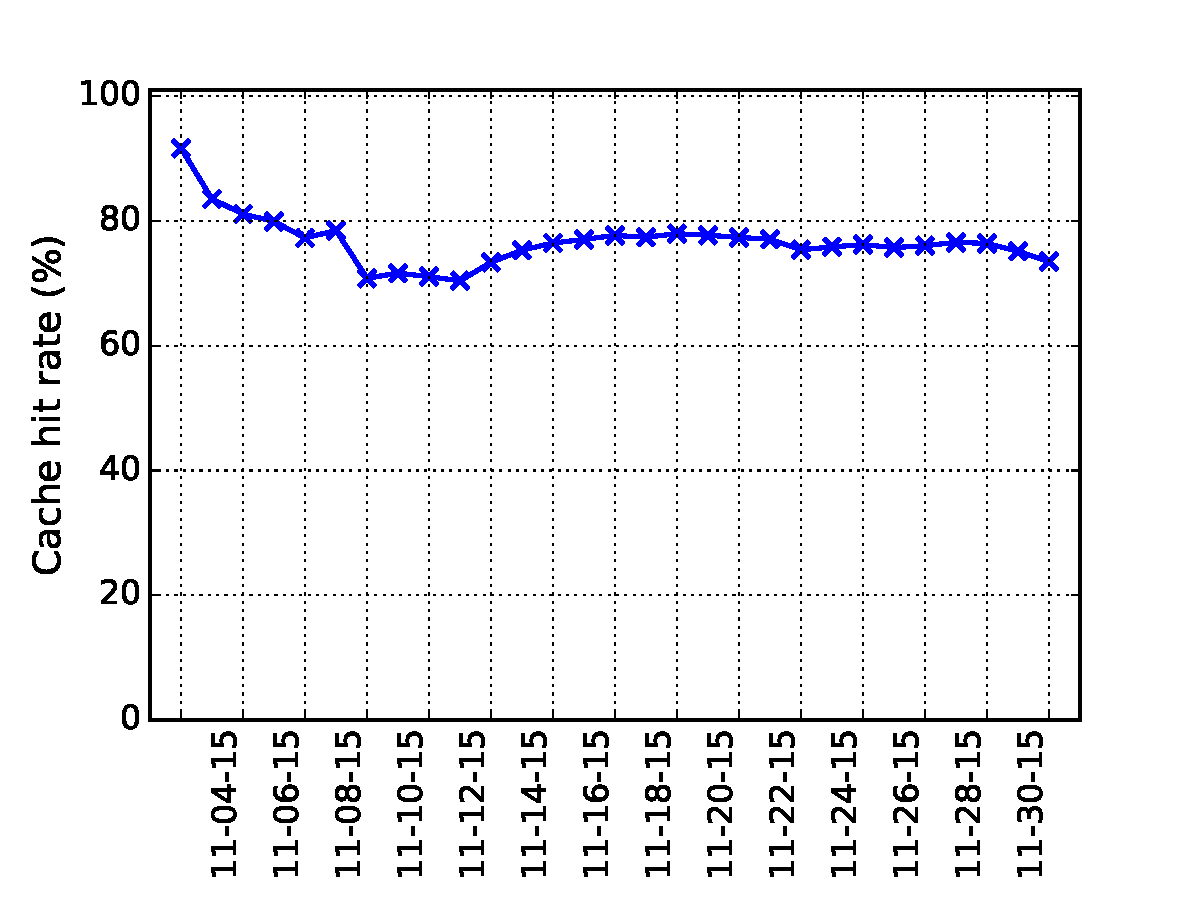
\includegraphics[width=2.5in]{figure/LRU_day}
\caption{Cache hit rate when updating cache content once a day.}
\label{fig:batchcache}
\end{center}
\end{figure}

We then investigate whether there is time locality for malwares.
Specifically, we hypothesize that malwares in the same family would appear in bursts.  
We borrow the cache mechanism from system research area to validate our hypothesis. 
Cache was previously used to predict bugs~\cite{predicting}, 
since bugs are introduced not uniformly in time but in bursts and with a strong time locality. 
We view malware submission reports as a stream according to each report's submission timestamp, and feed the stream into a cache. 
If the cache hit rate is high, 
we can conclude that the appearance of malwares also has time locality. 

There are several notions in cache terminology: 
block size is defined as how many entries would be added into the cache or evicted from the cache together.
Pre-fetch means loading entries that the cache has not encountered yet. 
Replacement policy controls how to evict entries from cache, when the cache is full. 
We use the most simple cache setting in our evaluation. We fix the block size to be 1, disable pre-fetch, 
and use LRU (least recently used) replacement policy.
Our malware family cache works as follows.

We start with an empty cache. 
For a new malware submission, if the malware family is already in the cache, 
we will move the related cache entry to the front of our cache entry list. 
If the new malware family is not in the cache, 
we will create a new cache entry and add it into the front of our cache entry list. 
If our cache is full, we need to evict the entry at the end. 
The cache hit rate is calculated as follows: 

$$ \mbox{hit rate} = \dfrac{\mbox{\# of hits}}{\mbox{\# of hits + \# of misses}}$$



We implement the LRU cache by using
python-2.7. Our experiment is conducted on an aws c4.4xlarge virtual machine, 
which contains 16 virtual cpus and 30G memory.

We conduct two experiments. In the first experiment, 
we explore how the cache hit rate changes with the number of cache entries. 
We change the cache size from 10 to 1000. As shown in Figure~\ref{fig:cache}, 
the hit rate grows from 69.29\% to 98.14\%. 
When using more than 80 cache entries, which is less than 1\% of the total number of malware families, the cache hit rate rises above 90\%, 
and when using more than 230 cache entries, which is less than 3\% of the total number of malware families, 
the cache hit rate rises above 95\%. 

In the second experiment, we fix the cache size at 100, 
and we lower the cache content update frequency from once per malware report to once per day, 
that is, we keep cache content unchanged to count cache hits and cache misses each day and update the cache content at the end of each day.
Figure~\ref{fig:batchcache} shows the cache hit rate for each day. 
Most cache hit rate falls in a range between 70\% and 80\%.  


{\bf Observation 2:} 
The appearance of malwares in each family has a strong time locality.  

\underline{Discussion.}
Resources to combat malwares are limited. 
Any techniques that could allow antivirus vendors to focus their efforts would be great. 
Our cache-based malware prediction technique can predict which malware families will appear in the near future with high precision. 
We note that there are many other cache configurations, for example, those
with different cache block sizes, different pre-fetch mechanisms, 
and different replacement policies. 
We leave the exploration of the effect of their combinations for the future. 
Currently, we use malware family as prediction granularity. 
In the future, we could try to predict malwares using a finer granularity. 
For example, ssdeep values are also provided in VirusTotal metadata, 
and these values can be used to cluster malwares. 
We could cluster malwares in each family first, and then use cluster as prediction granularity. 
